\section{Przegląd rozwiązań}
  Na przestrzeni ostatnich paru lat pojawiło się wiele rozwiązań zastosowania
  sieci neuronowych do edycji obrazu, duża część z nich była przełomowa w
  swojej dziedzinie. Powstawały rewolucyjne architektury sieci oraz technologie
  z nimi związane. Takie cechy sieci jak niezwykła zdolność do generalizacji zdobytej wiedzy na nowe przypadki oraz olbrzymia elastyczność sprawiły, że
  znalazły one wiele rzeczywistych zastosowań.

  W tym rozdziale skupiono się na przedstawieniu kilku interesujących rozwiązań
  dla omawianej problematyki.
   Neuronowe sieci splotowe (CNN) stanowią podstawową strukturę w zkaresie przetwarzania i analizowania obrazów cyfrowych. Stanowią podwaliny większości klasyfikatorów, detektorów, czy sieci segmentujących.

   Autorzy jednego z artykułów traktujących o sieciach splotowych \cite{cnn} opisują je następująco: "CNN to skuteczny algorytm poznawczy, stosowany powszechnie przy rozpoznawaniu wzorców i przetwarzaniu obrazów. Posiada wiele cech, takich jak prosta struktura, mniej parametrów treningowych, czy zdolność do adaptacji. CNN stały się gorącym tematem w zakresie analizy głosu i rozpoznawania obrazu. Ich struktura oparta na podziale wag czyni je bardziej podobnymi do biologicznych sieci neuronowych. Redukuje to złożoność modelu sieci oraz liczbę wag".

   Na CNN składają się zazwyczaj trzy rodzaje warstw, z których każda posiada inne cechy.

   Podstawową warstwę stanowi warstwa splotowa. Składa się ona ze zbioru filtrów (neuronów) odpowiedzialnych za ekstrakcję cech z analizowanych obrazów. Każda kolejna warstwa splotowa wydobywa z obrazu cechy o wyższych poziomach abstrakcji bazując na wynikach obliczeń poprzednich warstw tego rodzaju.

   Drugim istotnym elementem sieci splotowych jest warstwa poolingu. %TODO wstawić cytat

   Końcowy element CNN w większości przypadków stanowią warstwy gęste (FC). Odpowiadają one za dokonanie odpowiedniej klasyfikacji obrazu na podstawie danych dostarczonych przez warstwy poprzedzające. Są przez to nieodzowne w przypdaku zadań związanych z wszelkiego rodzaju klasyfikacją obrazów.

   Wymienione tutaj elementy składowe sieci splotowych mogą przyjmować różne rozmiary, powielać się, zmieniać miejscami i łączyć ze sobą. Zapewnia to szerokie pole do eksperymentów i sprawia, że sieci te zdolne są rozwiązywać złożone, różnorodne problemy z wielu dziedzin codziennego życia.

  \subsection{Colorful image colorization}

    Wraz z rozwojem sieci neuronowych, rosło zainteresowanie możliwościami zastosowania
    ich do kolorowania czarno-białych obrazów. Jedno z dostępnych rozwiązań tego
    zagadnienia zostało przedstawione przez grupę pracowników Uniwersytetu w
    Berkeley \cite{colorful_image_colorization}. Zamiarem ich pracy było stworzenie
    modelu, który niekoniecznie odtwarza oryginalne barwy obrazu, ale generuje
    barwy prawdopodbne, zdolne przekonać ludzkiego obserwatora o autentyczności
    obrazu. Uzyskane rezultaty zostały przedstawione na
    Rysunku \ref{fig:colorful_image_colorization}.

    \begin{figure}[ht]
      \centering
      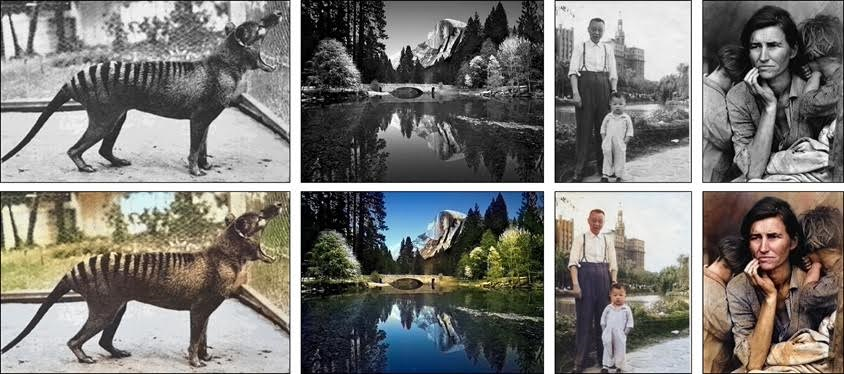
\includegraphics[width=4in]{image_colorization}
      \caption{Efekt kolorowanie czarno-białych zdjęć przez wytrenowany model.}
      \label{fig:colorful_image_colorization}
    \end{figure}

    Wykorzystany model składa się z wielu warstw CNN, w których skład wchodzą
    warstwa filtrów konwolucyjnych, warstwa ReLU (ang. Rectified
    Linear Unit) oraz warstwa BatchNorm (ang. Batch normalization).
    Aby zapobiec utracie informacji przestrzennych, sieć nie posiada warstw łączących.
    Istotny był także sposób
    przygotowania zbioru danych do trenowania modelu. Obrazy ze zbioru uczącego
    były wpierw konwertowane do modelu YUV, a następnie kanał Y był podawany na
    wejście modelu, warstwy UV pełniły funkcję pożądanej odpowiedzi w uczeniu
    nadzorowanym.

    Ważnym aspektem zbadanym w artykule było także dobranie odpowiedniej
    funkcji kosztu. Nieodpowiedni wybór skutkował desaturacją kolorowanych
    obrazów, jedną z potencjalnych przyczyn tego zjawiska może być tendencja
    sieci do tworzenia bardziej konserwatywnych odpowiedzi. Aby zniwelować ten
    efekt w modelu została zastosowana specjalna technika modyfikacji
    funkcji kosztu. Polega ona na przewidywaniu dystrybucji możliwych kolorów
    dla każdego piksela i zmienianiu kosztu dla modelu, w celu wyróżnienia rzadko
    spotykanych kolorów.

    Powstałe rozwiązanie dowodzi olbrzymiego potencjału zastosowanie sieci
    neuronowych w dziedzinie pracy nad obrazami.

  \subsection{Image Style Transfer Using Convolutional Neural Networks}
    W roku 2016 został przedstawiony światu A Neural Algorithm of Artistic Style
    \cite{image_style_transfer}. Wprowadzał on przełom w dziedzinie przenoszenia
    stylu jednego obrazu na inny, a jego sukces opierał się na właściwym wykorzystaniu
    konwolucyjnych sieci neuronowych. Podstawą tego sukcesu było odkrycie przez
    Leona A. Gatys oraz jego współpracowników, że w CNN reprezentacja treści
    obrazu oraz jego stylu jest rozłączna. Umożliwia to wydobycie stylu
    przetwarzanego obrazu oraz połączenie go z treścią innego obrazu, czego
    dokonuje właśnie A Neural Algorithm of Artistic Style. Rezultaty takich
    operacji można zaobserwować na Rysunku \ref{fig:image_style_transfer}

    \begin{figure}[ht]
      \centering
      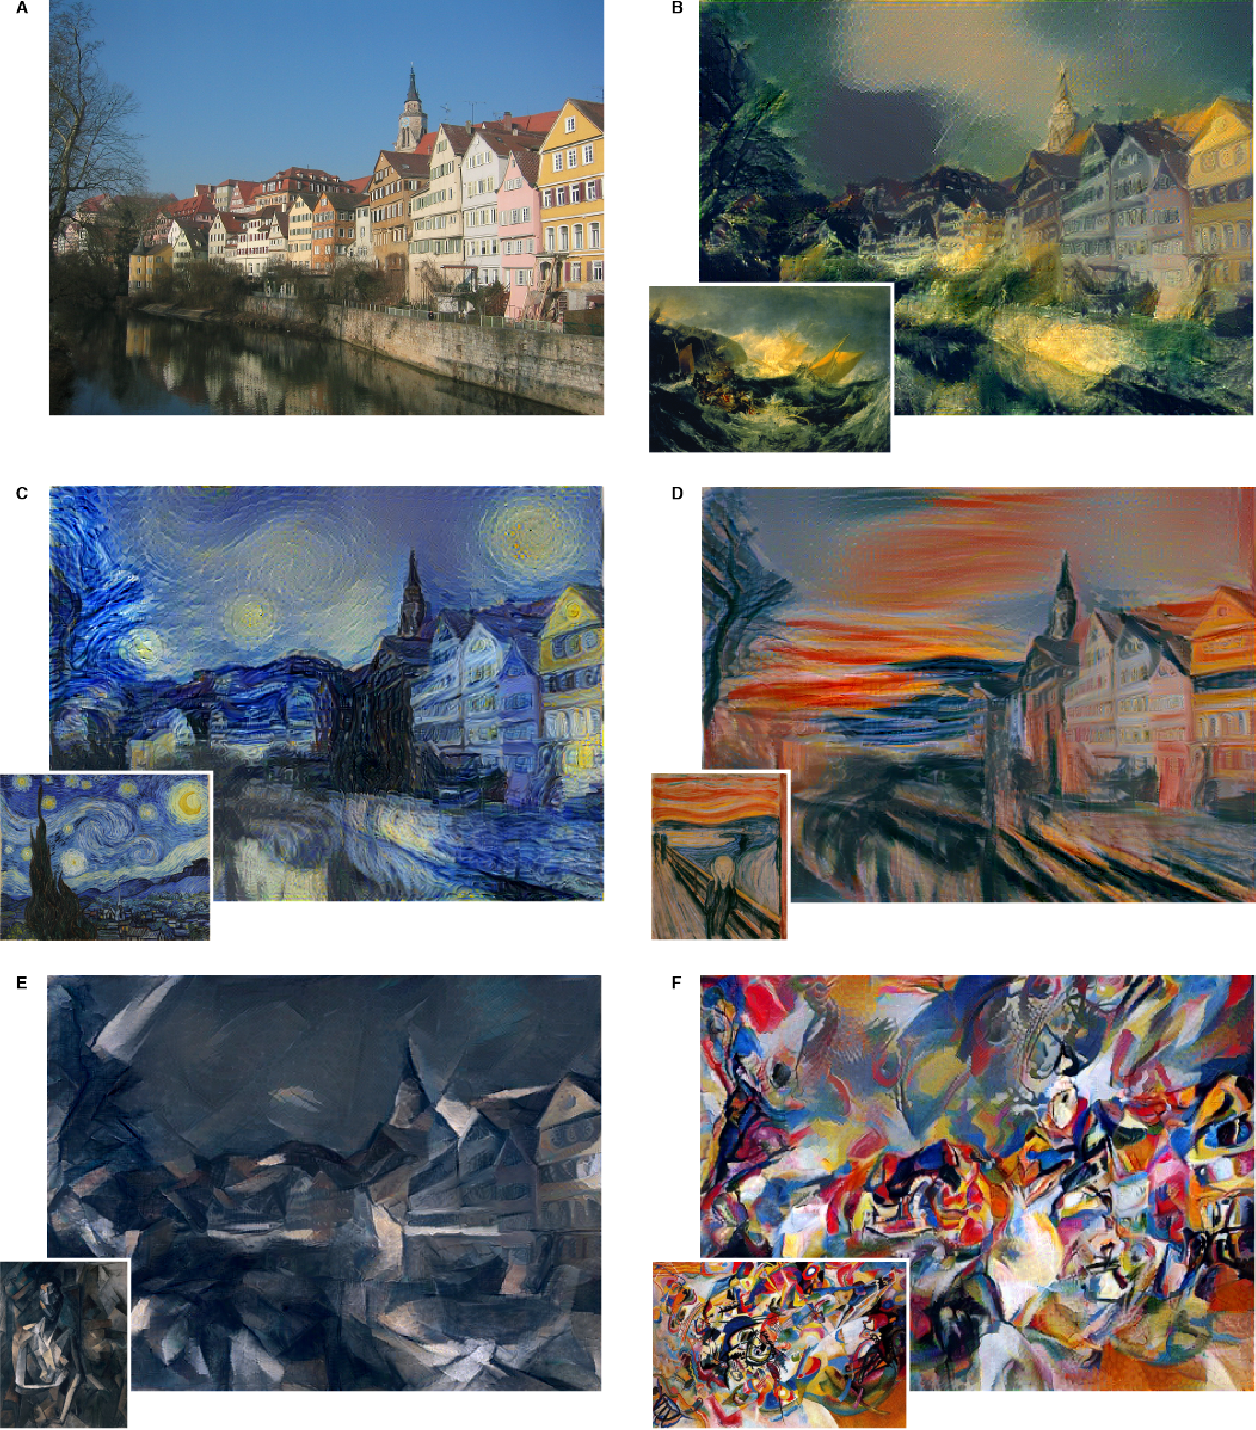
\includegraphics[width=4in]{image_style_transfer}
      \caption{Obrazy będące kombinacją treści zdjęcia ze stylami kilku znanych dzieł sztuki.}
      \label{fig:image_style_transfer}
    \end{figure}

    Do zbudowania modelu zostały użyte warstwy konwolucyjne oraz łączące z
    architektury VGG-Network \cite{vgg_network}, która została wytrenowana pod
    kątem rozpoznawanie obiektów i określania ich położenia. Dzięki temu sieć
    przetwarzając obraz tworzy jego reprezentację, która wraz z
    kolejnymi warstwami, przedstawia coraz wyraźniejszą informację o obiektach,
    a niekoniecznie o dokładnym wyglądzie obrazu.
    W modelu nie została użyta ani jedna warstwa gęsta, dzięki czemu na wyjściu
    możliwe jest otrzymanie dwuwymiarowego obrazu.
    Dla lepszej syntezy obrazów, w warstwach
    łączących zastosowano próbkowanie wartością średnią zamiast maksymalną.
    Takie zabiegi umożliwiają wyliczenie reprezentacji stylu z korelacji
    pomiędzy różnymi cechami w różnych warstwach konwolucyjnych.

    Cały proces renderowania polega na odpowiednim zapisaniu w modelu treści
    oraz stylu obrazów otrzymanych przez wcześniejsze podanie na model tychże
    obrazów. Wpierw obraz, z którego pobierany jest styl, jest podawany na
    wejście sieci oraz przeliczany, reprezentacja stylu wyselekcjonowana z
    właściwych warstw jest przechowywana, obraz z treścią jest poddawany temu samemu
    procesowi, ale reprezentacja treści jest wyciągana z ostatnich
    warstw konwolucyjnych.
    W celu uzyskania fuzji obrazów, zapisane reprezentacje treści i stylu są
    zapisywane w tych warstwach modelu skąd zostały odczytane, a następnie na wejście
    podawany jest obraz składający się z losowego szumu białego.
    Następnie poprzez iteracyjną minimalizację funkcji kosztu, obraz wejściowy jest modyfikowany, co w rezultacie końcowym doprowadza do nałożenia zapisanego
    stylu na wczytaną treść.

    A Neural Algorithm of Artistic Style jest świetnym przykładem, jak elastyczne
    mogą być interfejsy do modyfikacji obrazu oparte na technologii sieci neuronowych.

  \subsection{Invertible Conditional GANs for image editing}
    Edycja obrazów może być dokonywana na wielu różnych poziomach zaawansowania
    i abstrakcji, operacje takie jak nakładanie filtrów mogą być
    wykonywane przez proste algorytmy. Jednak w przypadku próby modyfikacji
    elementów na obrazie, algorytmy te nie będą w stanie dokonać semantycznych
    zmian ze względu na brak możliwości zrozumienia treści obrazu. Rozwiązanie
    tego problemu zostało przedstawione w postaci modelu IcGAN
    (ang. Invertible Conditional Generative Adversarial Network) w roku 2016
    \cite{gan_editing}. Zaprezentowany model był to enkoder z możliwością
    generowania wektora informacji o atrybutach obrazu połączony z warunkowym
    GAN zdolnym do kontrolowania cech generowanych obrazów na podstawie dodatkowej
    informacji warunkowej. Takie działanie umożliwia wprowadzania zmian w
    atrybutach generowanego obrazu uzyskiwanego na wyjście cGAN (ang. conditional Generative
    Adversarial Network). Rezultaty działania modelu można zaobserwować na
    Rysunku \ref{fig:IcGAN}

    \begin{figure}[ht]
      \centering
      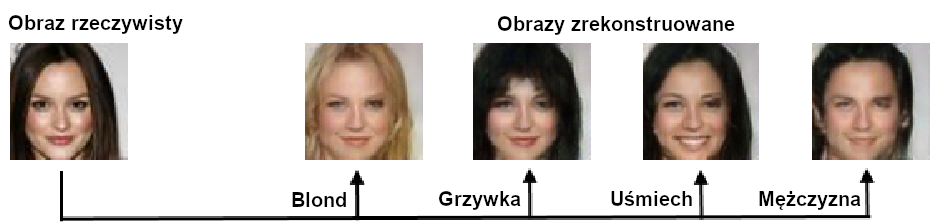
\includegraphics[width=4in]{IcGAN}
      \caption{Obrazy generowane przez IcGAN.}
      \label{fig:IcGAN}
    \end{figure}

    Wykorzystany w IcGAN Ekonder w rzeczywistości składa się z dwóch podrzędznych
    Enkoderów, Enkoder $E_{z}$ koduje wejściowy obraz do utajonego wektora $z$ reprezentacji
    obrazu, natomiast Enkoder $E_{y}$ generuje wektor informacji $y$ oddających
    pewne kluczowe atrybuty obrazu. Enkodey są trenowane z użyciem już wytrenowanego
    cGAN oraz obrazów rzeczywistych z etykietami ze zbioru uczącego. Zbadane
    zostały także różne podejścia interakcji między dwoma Enkoderami, wyróżnić
    można podejście, w którym Enkdodery są w pełni niezależne, podejście
    gdzie wyjście $E_{z}$ jest zależne od wyjścia $E_{y}$, a także podejście
    gdzie $E_{z}$ oraz $E_{y}$ są połączone w jednej Enkoder o współdzielonych
    warstwach i dwóch wyjściach.

    W przypadku cGAN możemy wyróżnić dwa najważniejsze czynniki, które trzeba
    mieć na uwadze. Pierwszym jest źródło wektora $y$ podawanego na
    Generator. W przypadku Dyskryminatora $y$ jest pobierany ze
    zbioru treningowego, jednakże w przypadku podawania tego
    samego wektora na Generator wystąpiła możliwość, że może dojść do niepożądanego
    przeuczenia modelu. Autorzy artykułu dokonali analizy tego rozwiązania,
    a także zbadali wydajność metody Bezpośredniej Interpolacji oraz
    Jądrowego estymatora gęstości. Wynikiem tych badań było stwierdzenie, że
    dla danej problematyki najlepiej sprawdza się podawanie wektora $y$ ze zbioru
    uczącego, możliwość przeuczenia modelu została skomentowana następująco:
    \begin{quote}
      % This is only likely to occur if the conditional information
      % is, to some extent, unique for each image. In the case where the attributes of an image are binary, one attribute vector y could describe a varied and large enough subset of images, preventing the model from overfitting given y.
      'Jest to możliwe tylko, gdy informacje warunkowe są do pewnego stopnia
      unikatowa dla każdego obrazu. W tym przypadku, gdzie atrybuty obrazów są
      binarne, jeden wektor $y$ może opisać wystarczająco duży i zróżnicowany
      podzbiór obrazów, zapobiegając nadmiernemu dopasowaniu się modelu do
      danego $y$.'
    \end{quote}
    Drugim czynnikiem jest warstwa Generatora i Dyskryminatora cGAN na
    którą podany jest wektor $y$. Guim Perarnau oraz jego współpracownicy ustalili, że najlepsze rezultaty otrzymuje się po podaniu wektora $y$ na warstwę wejściową
    Generatora oraz pierwszą warstwę konwolucyjną Dyskryminatora.

    Ważnym spostrzeżeniem z analizy rozwiązania IcGAN jest obecność
    olbrzymiej ilości różnorodnych rozwiązań opartych na sieciach neuronowych,
    coraz to nowe architektury zostają wynalezione, aby udoskonalić
    zastosowania sieci neuronowych do przetwarzania i modyfikowania obrazów.

  \subsection{Neural photo editing}
    W 2017 roku Andrew Brock, Theodore Lim, J.M. Ritchie and Nick Weston
    zaprezentowali Neural Photo Editor \cite{neural_photo_editor}, narzędzie
    do edytowania obrazu wyposażone w mechanizmy wykrywania kontekstu zmiany.
    Twórcy opisują swój twór następująco:

    \begin{quote}
      % 'An interface that leverages the power of generative neural networks to
      % make large, semantically coherent changes to existing images.'
      'Interfejs wykorzystujący moc generatywnych sieci neuronowych do
      wprowadzania dużych, semantycznie spójnych zmian w istniejących obrazach.'
    \end{quote}

    Użytkowanie wygląda następująco: użytkownik pędzlem o określonym kolorze i
    rozmiarze maluje na wybranym obrazie, jednak zamiast zmieniać wartości
    pojedynczych pikseli, interfejs odczytuje kontekst edycji i wprowadza zmiany
    semantyczne w kontekście żądanej zmiany koloru. Efekt działania interfejsu
    został przedstawiony na Rysunku \ref{fig:npe}.

    \begin{figure}[ht]
      \centering
      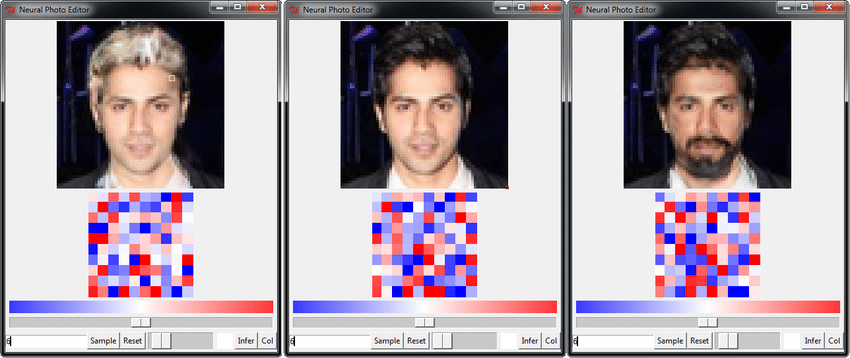
\includegraphics[width=4in]{NPE}
      \caption{Efekt działania Neural Photo Editor.}
      \label{fig:npe}
    \end{figure}

    Skuteczność NPE (Neural Photo Editor) polega na zastosowaniu IAN
    (ang. Introspective Adversarial Network), czyli sieci złożonej z połączonych
    VAE (ang. Variational Autoencoder) \cite{vae} oraz GAN, w taki sposób, że dekodująca
    sieć autoenkodera jest używana jako sieć generująca w GAN.
    Poprzez przechwytywanie przez model dalekosiężnych zależności, wykorzystanie
    bloku obliczeniowego bazującego na rozszerzonych splotach o
    współdzielonych wagach oraz dzięki zastosowaniu ulepszonej generalizacji,
    udało się osiągnąć dokładną rekonstrukcje obrazu bez strat na jakości detali.

    Powstanie NPE utwierdza w przekonaniu, że aktualne możliwości sieci
    neuronowych do edycji obrazu znacznie przewyższają zwykłe algorytmy pod
    względem możliwości oraz uzależnienia od wkładu ludzkiego.


  \subsection{Face App}
